\begin{frame}
\frametitle{5.6 (August 2016)}
\begin{block}{OTB}
\begin{itemize}
\item MPI pipeline execution
\item Samples extractor and selection for supervised classification
\item Improve classification on vector
\item Support for Sentinel-1 products (geometric calibration)
\end{itemize}
\end{block}

\begin{block}{Monteverdi 3.4}
\begin{itemize}
\item Improve OTB-applications display \& search bar
\end{itemize}
\end{block}
\end{frame}

\begin{frame}[fragile]
\frametitle{Parallel OTB pipeline with MPI}
  \begin{center}
  \vspace{-0.5cm}
  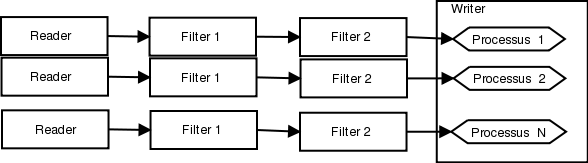
\includegraphics[width=0.6\textwidth]{images/mpi.png}
  \begin{scriptsize}
\begin{verbatim}
    $ mpirun -np $nb_procs --hostfile $PBS_NODEFILE  \
    otbcli_BundleToPerfectSensor \
    -inp $ROOT/IMG_PHR1A_P_001/IMG_PHR1A_P_201605260427149_ORT_1792732101-001_R1C1.JP2 \
    -inxs $ROOT/IMG_PHR1A_MS_002/IMG_PHR1A_MS_201605260427149_ORT_1792732101-002_R1C1.JP2 \
    -out $ROOT/pxs.tif uint16 -ram 1024

    ------------ JOB INFO 1043196.tu-adm01 -------------
    
    JOBID           : 1043196.tu-adm01
    USER            : michelj
    GROUP           : ctsiap
    JOB NAME        : OTB_mpi
    SESSION         : 631249
    RES REQSTED     : mem=1575000mb,ncpus=560,place=free,walltime=04:00:00
    RES USED        : cpupercent=1553,cput=00:56:12,mem=4784872kb,ncpus=560,vmem=18558416kb,
    walltime=00:04:35
    BILLING         : 42:46:40 (ncpus x walltime)
    QUEUE           : t72h
    ACCOUNT         : null
    JOB EXIT CODE   : 0
    
    ------------ END JOB INFO 1043196.tu-adm01 ---------
\end{verbatim}
\end{scriptsize}
\end{center}
\end{frame}
